\subsection{Revisiting the Simulations}

Now we can revisit our simulations with a much more efficient simulation function.
This time, we simulate over $1$ million randomly generated pools, producing the results in \Cref{Figure:simulation-updated-results-histogram}.
\begin{figure}[htbp]
    \centering
    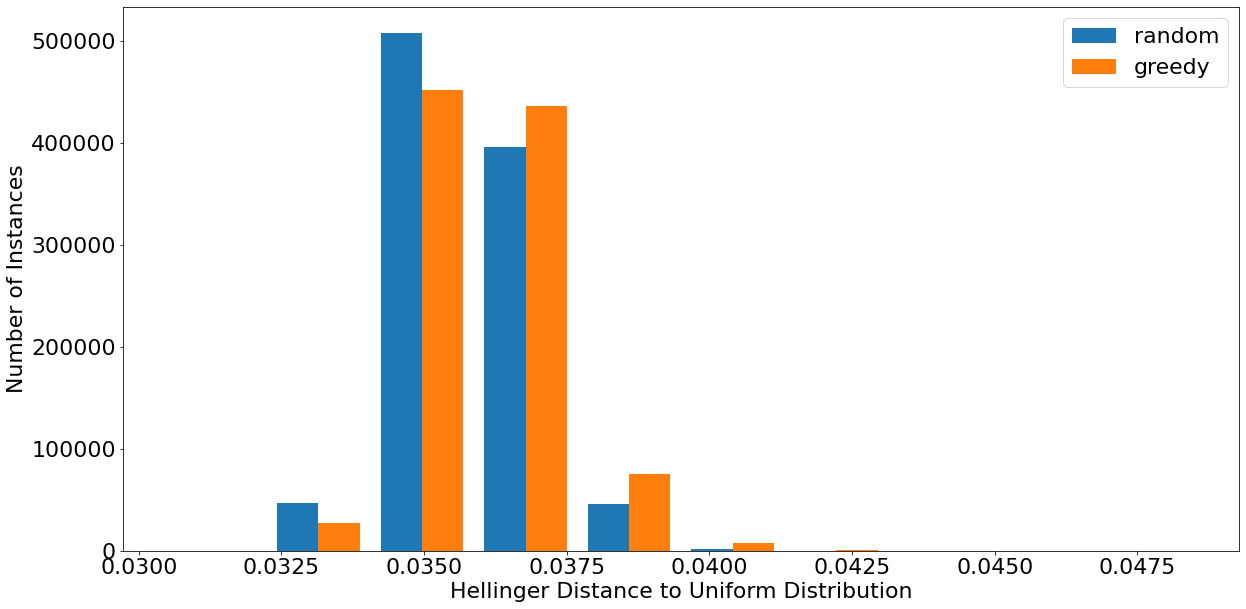
\includegraphics[width=.9\textwidth]{figures/simulations-updated.png}
    \caption{Hellinger distance of distributions produced by ARAMNet to the uniform distribution using random and greedy ordering}
    \label{Figure:simulation-updated-results-histogram}
\end{figure}
As a side remark, the reader may notice that in \Cref{Figure:simulation-updated-results-histogram} the distance to the uniform distribution is higher than in \Cref{Figure:simulation-results-histogram}.
This is expected since ARAMNet has ${\sim}0.0325$ validation loss.

\Cref{Figure:simulation-updated-results-histogram} shows that the greedy ordering produces distributions that have larger distance to the uniform distribution than when using a random ordering.
Indeed, the mean Hellinger distance to the uniform distribution is $0.03578$ when using a random ordering and $0.03603$ when using a greedy ordering.
Now, we can be a bit more sure that the phenomena we saw in \Cref{Section:Initial-Simulations} was not due to a small sample size.
In fact, it may actually be the case that the greedy ordering is not as optimal as we conjectured.
This doesn't quite disprove our conjecture since all of this evidence is empirical, but it does suggest that there may be other mechanisms at play within the player orderings.
